\documentclass{standalone}
\usepackage{tikz}

\usetikzlibrary{positioning}
\usetikzlibrary{decorations.pathmorphing}

\tikzset{snake it/.style={decorate, decoration={snake, segment length=1.5mm, amplitude=0.5mm}}}
\tikzset{
    position/.style args={#1:#2 from #3}{
        at=(#3.#1), anchor=#1+180, shift=(#1:#2)
    }
}

\begin{document}
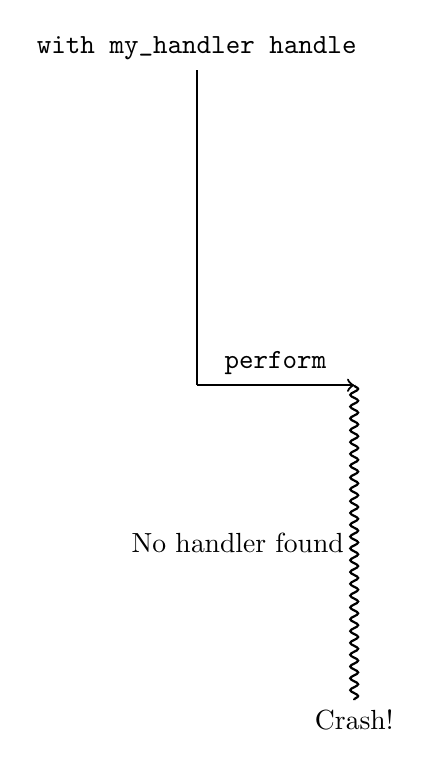
\begin{tikzpicture}
    \draw[thick] (0, 0) -- (0, -4)
        node[at start, above]{\verb|with my_handler handle|};
    \draw[->, thick] (0, -4) -- (2, -4)
        node[midway, above]
        {\verb|perform|};
    \draw[thick, snake it] (2, -4) -- (2, -8)
        node[left, midway]{No handler found}
        node[at end, below]{Crash!};
    
    % \draw[help lines] (0,0) grid (10,-10);
\end{tikzpicture}
\end{document}